\section{离散信道及其容量}

\begin{remarkBox}{本章重点}
本章主要回答“一个离散信道最多能可靠传多少信息”这个问题。学习时先把信道看成从输入随机变量 $X$ 到输出随机变量 $Y$ 的概率映射，再掌握转移概率矩阵、信道容量 $C=\max_{p(x)}I(X;Y)$，最后会计算无噪信道、对称信道和级联信道的容量。
\end{remarkBox}

本章的主线很简单：先把信道抽象成输入 $X$ 到输出 $Y$ 的概率映射，再用 $p(y\mid x)$ 或转移矩阵 $[P]$ 描述这种映射；接着通过最大化平均互信息得到信道容量；最后在无噪信道、对称信道和级联信道这些典型结构中直接计算容量。做题时最重要的是识别信道类型、写对矩阵方向、判断是否对称，以及在级联信道中按顺序做矩阵乘法。

\subsection{离散信道概述}

信道是信号传输的媒介，是连接发送端和接收端的物理通道。信息论并不直接研究具体电缆、无线电波或调制电路，而是把信道抽象成一个概率模型：输入给定后，输出以某种条件概率出现。

\begin{definitionBox}{信道}
信道是从输入端向输出端传送信息的系统。若输入随机变量为 $X$，输出随机变量为 $Y$，则信道的统计特性由条件概率 $p(y\mid x)$ 描述。
\end{definitionBox}

信道可以从多个角度分类。按输入、输出取值，可分为\textbf{离散信道}、\textbf{连续信道}、\textbf{半连续信道}和\textbf{时间离散连续信道}；按输入、输出端个数，可分为\textbf{单用户信道}和\textbf{多用户信道}，其中多用户信道包括多元接入信道和广播信道；按转移概率性质，可分为\textbf{无噪声信道}、\textbf{有噪声信道}、\textbf{无记忆信道}和\textbf{有记忆信道}。还可以按统计特性分为恒参信道和变参信道，按噪声性质分为高斯噪声信道和非高斯噪声信道。

这些分类不是为了背名词，而是为了判断后面该用哪种模型和哪种容量公式。研究信道的核心，是回答信息怎样才能\textbf{有效}、\textbf{可靠}地传输；信道容量给出的就是固定信道能够支持的最大信息传输能力。

\subsection{离散信道的数学模型}

\subsubsection{离散无记忆信道}
一般的 $N$ 符号离散信道可以写成
\[
\{X^N,p(y^N\mid x^N),Y^N\},
\]
其中 $x^N=(x_1,x_2,\dots,x_N)$，$y^N=(y_1,y_2,\dots,y_N)$。若当前输出只依赖当前输入，而不依赖过去的输入输出，就得到离散无记忆信道。

\begin{definitionBox}{离散无记忆信道}
若信道转移概率满足
\[
p(y^N\mid x^N)=\prod_{n=1}^{N}p(y_n\mid x_n),
\]
则称该信道为\textbf{离散无记忆信道}（DMC）。
\end{definitionBox}

\begin{definitionBox}{平稳离散无记忆信道}
若对任意时刻 $m,n$，都有
\[
p(y_n=b_j\mid x_n=a_i)=p(y_m=b_j\mid x_m=a_i),
\]
则称该离散无记忆信道为\textbf{平稳信道}或\textbf{恒参信道}。此时信道可简化为单符号模型
\[
\{X,p(y\mid x),Y\}.
\]
\end{definitionBox}

\subsubsection{转移概率矩阵}

设输入字母表为 $A=\{a_1,a_2,\dots,a_r\}$，输出字母表为 $B=\{b_1,b_2,\dots,b_s\}$。单符号离散信道由条件概率
\[
p_{ij}=p(y=b_j\mid x=a_i)
\]
完全描述。

信道转移概率矩阵为
\[
[P]=
\begin{bmatrix}
p_{11}&p_{12}&\cdots&p_{1s}\\
p_{21}&p_{22}&\cdots&p_{2s}\\
\vdots&\vdots&\ddots&\vdots\\
p_{r1}&p_{r2}&\cdots&p_{rs}
\end{bmatrix},
\qquad
p_{ij}\ge0,
\quad \sum_{j=1}^{s}p_{ij}=1.
\]
矩阵的每一行对应一个输入符号，每一列对应一个输出符号。

\begin{warningBox}{矩阵方向}
本章约定 $p_{ij}=p(y=b_j\mid x=a_i)$，即\textbf{行是输入，列是输出}。做题时先写清输入、输出字母表，避免把矩阵转置。
\end{warningBox}

\begin{example}
\textbf{二元对称信道（BSC）}：输入、输出字母表均为 $\{0,1\}$，错误率为 $\epsilon$。写出转移概率矩阵并画出转移图。

\noindent \textbf{解题流程}：\\[2pt]
步骤一：正确传输概率为 $1-\epsilon$。\\
步骤二：错误传输概率为 $\epsilon$。\\
步骤三：按“行输入、列输出”写矩阵。

\textbf{解}：
\[
[P]=\begin{bmatrix}
1-\epsilon & \epsilon\\
\epsilon & 1-\epsilon
\end{bmatrix}.
\]

\begin{center}
\begin{tikzpicture}[
    scale=1.0,
    node/.style={draw, circle, minimum size=0.72cm, fill=RoyalBlue!8},
    edge label/.style={font=\scriptsize, fill=white, inner sep=1pt}
  ]
  \node[node] (x0) at (0,1.2) {$0$};
  \node[node] (x1) at (0,-1.2) {$1$};
  \node[node] (y0) at (4,1.2) {$0$};
  \node[node] (y1) at (4,-1.2) {$1$};
  \draw[->] (x0) -- node[edge label, above] {$1-\epsilon$} (y0);
  \draw[->] (x1) -- node[edge label, below] {$1-\epsilon$} (y1);
  \draw[->] (x0) -- node[edge label, above right] {$\epsilon$} (y1);
  \draw[->] (x1) -- node[edge label, below right] {$\epsilon$} (y0);
  \node[font=\scriptsize] at (0,2.0) {输入};
  \node[font=\scriptsize] at (4,2.0) {输出};
\end{tikzpicture}
\end{center}
\end{example}

\begin{example}
\textbf{二元删除信道}：输入字母表 $A=\{0,1\}$，输出字母表 $B=\{0,2,1\}$。设 $0$ 被正确接收为 $0$ 的概率为 $p$，被删除为 $2$ 的概率为 $1-p$；$1$ 被删除为 $2$ 的概率为 $1-q$，被正确接收为 $1$ 的概率为 $q$。求转移矩阵。

\textbf{解}：按输出顺序 $0,2,1$ 排列列，则
\[
[P]=\begin{bmatrix}
p&1-p&0\\
0&1-q&q
\end{bmatrix}.
\]
\end{example}

\subsection{信道容量的定义}

\subsubsection{容量的含义}
对一个固定信道，转移概率 $p(y\mid x)$ 已经给定；但输入分布 $p(x)$ 可以选择。不同输入分布会产生不同的平均互信息 $I(X;Y)$，其中最大值就是信道容量。

\begin{definitionBox}{信道容量}
平稳离散无记忆信道的容量定义为
\[
C=\max_{p(x)} I(X;Y).
\]
单位为 bit/信道符号（若对数底为 $e$，单位为 nat/信道符号）。
\end{definitionBox}

信道容量 $C$ 是信道传输最大信息速率能力的度量。信道一旦给定，$p(y\mid x)$ 固定，因此 $C$ 只由信道本身决定，而不是由某一个随便选定的输入分布决定。

\begin{warningBox}{容量与输入分布}
“$C$ 与 $p(x)$ 无关”不是说计算时不用考虑 $p(x)$，而是说容量已经对 $p(x)$ 取了最大值。对一般信道，达到容量的输入分布不一定等概；对对称信道，等概输入可以达到容量。
\end{warningBox}

若信道输入、输出为 $N$ 维随机矢量 $X^N,Y^N$，常用每个信道符号的容量表示为
\[
C=\max_{p(x_1,\dots,x_N)}\frac{1}{N}I(X^N;Y^N).
\]

可以把信道想象成水管：水管本身的粗细和形状对应 $p(y\mid x)$，水龙头怎么开对应 $p(x)$，实际水流速度对应传输率 $R$，最大可达到的水流速度对应容量 $C$。这个类比的重点是区分“信道本身”和“输入如何使用信道”：容量是固定水管能达到的最大流速，而不是某一次随便打开水龙头得到的流速。

\subsection{离散无噪信道的容量}

离散无噪信道没有随机错误，但仍要区分不同的映射关系。考试中最容易混淆的是“无损”和“确定”：前者强调输出能反推输入，后者强调输入能确定输出。

三类无噪信道的区别可以按“由谁决定谁”来记：\textbf{无损信道}要求每个输出符号只对应一个输入符号，接收端能由输出确定输入；\textbf{确定信道}要求每个输入符号只对应一个输出符号；\textbf{无扰信道}则要求输入与输出一一对应，既无损又确定。

\begin{formulaBox}{离散无噪信道容量}
设输入符号数为 $r$，有效输出符号数为 $s$：
\[
\text{无损信道：}\quad C=\max H(X)=\log r,
\]
\[
\text{确定信道：}\quad C=\max H(Y)=\log s,
\]
\[
\text{无扰信道：}\quad C=\log r=\log s.
\]
\end{formulaBox}

无损信道允许一个输入对应多个输出，但每个输出只能来自一个输入；确定信道允许多个输入对应同一个输出，但每个输入只能产生一个输出。两者关注方向不同。

\subsection{离散对称信道的容量}

\subsubsection{对称信道的判断}
对称信道是本章最重要的可直接套公式的信道类型。它的好处是：不需要复杂优化，等概输入就能达到容量。

\begin{definitionBox}{离散对称信道}
若信道转移概率矩阵按输出列可分为若干子矩阵，每个子矩阵满足：每一行是其他行的置换，每一列是其他列的置换，则称该信道为\textbf{对称信道}。
\end{definitionBox}

若整个转移矩阵本身就是一个满足行置换、列置换条件的子矩阵，称为\textbf{强对称信道}；若需要分成多个子矩阵后才满足条件，称为\textbf{准对称信道}或\textbf{弱对称信道}。

判断对称性时，先看每一行是否由同一组概率数置换得到，再看每一列是否也具有相同的列和结构。若整体满足这两个条件，就是强对称信道；若需要按输出列分成若干块后才分别满足，则是准对称信道。若各行的概率集合本身不同，通常就不是对称信道。

\begin{example}
\textbf{判断强对称信道}：判断矩阵
\[
[P]=\begin{bmatrix}
0.3&0.2&0.5\\
0.5&0.3&0.2\\
0.2&0.5&0.3
\end{bmatrix}
\]
是否为强对称信道。

\textbf{解}：每一行都是 $0.3,0.2,0.5$ 的置换；每一列也是相同概率集合的置换，因此该信道为强对称信道。
\end{example}

\subsubsection{对称信道容量公式}

\begin{theoremBox}{定理6.2：离散对称信道容量}
对离散对称信道，输入等概率时达到信道容量：
\[
C=H(Y)-H(p_1,p_2,\dots,p_s),
\]
其中 $H(Y)$ 为输入等概率时输出的熵，$H(p_1,p_2,\dots,p_s)$ 为转移概率矩阵某一行的熵。
\end{theoremBox}

若信道为强对称信道，输出符号数为 $s$，则输入等概时输出也等概，容量为
\[
C=\log s-H(p_{11},p_{12},\dots,p_{1s}).
\]

若 $r$ 元对称信道的错误概率为 $p$，每个错误输出平均分配概率 $p/(r-1)$，则
\[
C=\log r-H(p)-p\log(r-1).
\]
特别地，二元对称信道（BSC）容量为
\[
C=1-H(p).
\]

\begin{example}
\textbf{强对称信道容量}：信道转移矩阵为
\[
[P]=\begin{bmatrix}
1/2&1/3&1/6\\
1/6&1/2&1/3\\
1/3&1/6&1/2
\end{bmatrix}.
\]
求容量和达到容量时的输出分布。

\noindent \textbf{解题流程}：\\[2pt]
步骤一：判断矩阵为强对称。\\
步骤二：输入等概达到容量，输出也等概。\\
步骤三：用 $C=\log3-H(1/2,1/3,1/6)$。

\textbf{解}：达到容量时
\[
q_1=q_2=q_3=\frac13,
\]
因此
\[
C=\log_2 3-H\left(\frac12,\frac13,\frac16\right)\approx1.126\text{ bit/符号}.
\]
\end{example}

需要特别注意，等概输入达到容量只对对称信道可以直接使用。强对称信道在等概输入下输出也等概；准对称信道虽然等概输入达到容量，但输出分布不一定等概。

\subsection{级联信道及其容量}

\subsubsection{级联信道模型}
级联信道表示信息经过多个信道或处理环节逐步传递。直观上，后一级信道只能看到前一级输出，看不到更早的输入。

\begin{definitionBox}{级联信道}
若随机变量 $(X,Y,Z)$ 构成马氏链 $X\to Y\to Z$，即
\[
P(z\mid x,y)=P(z\mid y),
\]
则称信道 $X-Y$ 与 $Y-Z$ 构成\textbf{级联信道}。
\end{definitionBox}

\begin{center}
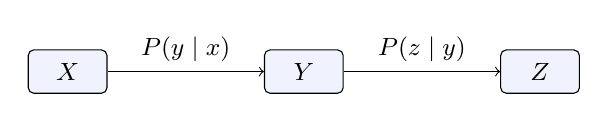
\begin{tikzpicture}[
    node/.style={draw, rounded corners=2pt, minimum width=1.0cm, minimum height=0.55cm, fill=RoyalBlue!8},
    every node/.style={font=\small}
  ]
  \node[node] (x) at (0,0) {$X$};
  \node[node] (y) at (3,0) {$Y$};
  \node[node] (z) at (6,0) {$Z$};
  \draw[->] (x) -- node[above] {$P(y\mid x)$} (y);
  \draw[->] (y) -- node[above] {$P(z\mid y)$} (z);
\end{tikzpicture}
\end{center}

若 $X-Y$ 的转移矩阵为 $P_{XY}$，$Y-Z$ 的转移矩阵为 $P_{YZ}$，则级联后的整体转移矩阵为
\[
P_{XZ}=P_{XY}P_{YZ}.
\]

\subsubsection{数据处理定理}

\begin{theoremBox}{定理6.3：马氏链中的信息不增}
若 $X,Y,Z$ 构成马氏链 $X\to Y\to Z$，则
\[
I(X;Z)\le I(X;Y),
\qquad
I(X;Z)\le I(Y;Z).
\]
\end{theoremBox}

\begin{theoremBox}{定理6.4：数据处理定理}
在通信系统中，若信源序列 $U^L$ 经编码器得到 $X^N$，通过信道得到 $Y^N$，再译码得到 $V^L$，则
\[
I(U^L;V^L)\le I(X^N;Y^N).
\]
\end{theoremBox}

数据处理定理的直觉是：处理不能凭空产生关于原始信源的新信息。信息经过编码器、信道、译码器等环节后，关于原信源的互信息只会不增；处理次数越多，通常信息损失越多。

\begin{example}
\textbf{两级 BSC 级联}：一个 BSC 的转移矩阵为
\[
P=\begin{bmatrix}1-\epsilon&\epsilon\\ \epsilon&1-\epsilon\end{bmatrix}.
\]
求两个相同 BSC 级联后的转移矩阵。

\textbf{解}：
\[
P^2=\begin{bmatrix}
(1-\epsilon)^2+\epsilon^2 & 2\epsilon(1-\epsilon)\\
2\epsilon(1-\epsilon)&(1-\epsilon)^2+\epsilon^2
\end{bmatrix}.
\]
因此两级级联仍是 BSC，其等效错误率为
\[
\epsilon_2=2\epsilon(1-\epsilon).
\]
若输入等概，则
\[
I(X;Y)=1-H(\epsilon),
\qquad
I(X;Z)=1-H(2\epsilon(1-\epsilon)).
\]
\end{example}

\begin{example}
\textbf{两级 BSC 容量}：若 BSC 错误率 $\epsilon=1/3$，求两级级联信道容量。

\textbf{解}：两级级联矩阵为
\[
P^2=\begin{bmatrix}
5/9&4/9\\
4/9&5/9
\end{bmatrix}.
\]
该信道为强对称信道，输入等概达到容量，输出也等概。因此
\[
C=\log_2 2-H\left(\frac{4}{9}\right)
=1-H\left(\frac49\right)
\approx0.0089\text{ bit/符号}.
\]
\end{example}

\subsection{题型整理：第六章常见计算}

\textbf{题型快速判断}：看到题目后先判断它属于哪类：
\begin{itemize}
  \item 给信道描述 $\to$ 判断离散/连续、无噪/有噪、无记忆/有记忆；
  \item 给转移图 $\to$ 写转移概率矩阵，并检查每行和为 1；
  \item 给矩阵问容量 $\to$ 先判断是否无噪或对称；
  \item 给 BSC 错误率 $p$ $\to$ 直接用 $C=1-H(p)$；
  \item 给两个信道串联 $\to$ 先做矩阵乘法，再判断新信道类型；
  \item 出现 $X\to Y\to Z$ $\to$ 优先考虑马氏链和数据处理定理。
\end{itemize}

\textbf{答题模板}：
\begin{enumerate}
  \item \textbf{写转移矩阵}：先列输入字母表和输出字母表，再按 $p_{ij}=p(b_j\mid a_i)$ 填矩阵，最后检查每行概率和为 1。
  \item \textbf{容量定义题}：写 $C=\max_{p(x)}I(X;Y)$，说明 $p(y\mid x)$ 固定，容量只由信道决定。
  \item \textbf{对称信道容量}：先说明行、列置换关系，再写输入等概达到容量，最后套 $C=H(Y)-H(\text{某行})$。
  \item \textbf{BSC 题}：识别错误率 $p$，直接写 $C=1-H(p)$；若是级联，先求等效错误率。
  \item \textbf{级联题}：按顺序相乘 $P_{XZ}=P_{XY}P_{YZ}$，再用新矩阵计算互信息或容量。
\end{enumerate}

\begin{warningBox}{第六章易错点汇总}
\begin{itemize}
  \item 信道容量只由 $p(y\mid x)$ 决定，但计算容量时仍要对 $p(x)$ 最大化；
  \item 不要默认等概输入一定达到容量，只有对称信道等特殊情形可以直接这样做；
  \item 马氏链 $X\to Y\to Z$ 表示 $P(z\mid x,y)=P(z\mid y)$，不是 $P(z\mid y)=P(z\mid x)$；
  \item 级联信道矩阵要按信道顺序相乘；
  \item 信道级联后容量和互信息不会增加；
  \item BSC 中的 $H(p)$ 是二元熵函数，不是概率 $p$ 本身；
  \item 强对称信道等概输入时输出等概，准对称信道不一定。
\end{itemize}
\end{warningBox}

\subsection{公式速查表}

{\scriptsize
\begin{tabularx}{\textwidth}{@{}l>{\raggedright\arraybackslash}X@{}}
\toprule
\textbf{类别} & \textbf{公式 / 核心结论} \\
\midrule
离散无记忆信道 & \textcolor{Red}{$p(y^N\mid x^N)=\prod_{n=1}^{N}p(y_n\mid x_n)$} \\
\midrule
转移矩阵元素 & \textcolor{Red}{$p_{ij}=p(y=b_j\mid x=a_i)$，且 $\sum_jp_{ij}=1$} \\
\midrule
信道容量定义 & \textcolor{Red}{$C=\max_{p(x)}I(X;Y)$} \\
\midrule
矢量信道容量 & $C=\max_{p(x_1,\dots,x_N)}\frac1N I(X^N;Y^N)$ \\
\midrule
无损信道容量 & \textcolor{Red}{$C=\log r$} \\
\midrule
确定信道容量 & \textcolor{Red}{$C=\log s$} \\
\midrule
强对称信道 & \textcolor{Red}{$C=\log s-H(p_{11},p_{12},\dots,p_{1s})$} \\
\midrule
BSC 容量 & \textcolor{Red}{$C=1-H(p)$} \\
\midrule
$r$ 元对称信道 & \textcolor{Red}{$C=\log r-H(p)-p\log(r-1)$} \\
\midrule
级联矩阵 & \textcolor{Red}{$P_{XZ}=P_{XY}P_{YZ}$} \\
\midrule
两级 BSC 等效错误率 & $\epsilon_2=2\epsilon(1-\epsilon)$ \\
\midrule
数据处理不等式 & \textcolor{Red}{$X\to Y\to Z\Rightarrow I(X;Z)\le I(X;Y)$} \\
\bottomrule
\end{tabularx}
}

\subsection{本章要求}
本章学习重点：
\begin{itemize}
  \item 理解信道分类和离散信道的概率模型；
  \item 会根据转移图写出信道转移概率矩阵；
  \item 掌握信道容量定义 $C=\max_{p(x)}I(X;Y)$；
  \item 会计算无损信道、确定信道、无扰信道容量；
  \item 会判断强对称信道和准对称信道，并套用容量公式；
  \item 熟练使用 BSC 容量公式 $C=1-H(p)$；
  \item 会用矩阵乘法求级联信道转移矩阵；
  \item 理解马氏链和数据处理定理的“信息不增”含义。
\end{itemize}
